% Title: Report LaTex File: Concept Development
% Auther: DC Eksteen
% Student Number: 22623906
% Contact: 22623906@sun.ac.za
% Date: 2022/09/22
% Version: 2.0

\chapter{Concept Design and Evaluation}
% Section overview:

This section aims to identify and refine any requirements that were required of the training platform, and then demonstrate and analyse a concept solution that will be expanded into the final delivered demonstration model in further sections.

Table \ref{tab:conditions} shows the user requirements that were derived from the project objectives and literature review. These user requirements are then analysed in Section \ref{sec:req} to determine the performance and functional engineering requirements.

\begin{table}[H]
	%\renewcommand{\arraystretch}{\tablestretch}
	\centering
	\caption{Derived User Requirements}
	\begin{tabularx}{\textwidth}{>{\raggedright UR~}p{1.5 cm} X >{\raggedright\arraybackslash}p{2cm}}
		\toprule
		\multicolumn{2}{c}{User Requirement} & Priority                                                   \\
		\midrule
		\newR{UR:zwift}                      & Connect with Zwift                             & Essential \\
		\newR{UR:sim}                        & Realistic Riding Simulation                    & Essential \\
		\newR{UR:weight}                     & Weight Should be Comparable to Market Products & High      \\
		\newR{UR:range}                      & Accept a Wide Range of Bicycles                & High      \\
		\newR{UR:measure}                    & Accurate Measured Training Data                & Medium    \\
		\newR{UR:price}                      & Less Expensive than Market Products            & High      \\
		\newR{UR:store}                      & Platform Easily Stored                         & Medium    \\
		\bottomrule
	\end{tabularx}
	\label{tab:conditions}
\end{table}

\setcounter{reqCount}{0}

\newpage

\section{Requirement Analysis}
\label{sec:req}

\begin{table}[H]
	\renewcommand{\arraystretch}{\tablestretch}
	\centering
	\caption{Functional Engineering Requirements}
	\begin{tabularx}{\textwidth}{>{\raggedright FER~}p{0.8 cm} X >{\centering\arraybackslash}p{1.7cm}}
		\toprule
		\multicolumn{2}{c}{Functional Requirement} & Reference                                                                                 \\
		\midrule
		\newR{FR:ble}                              & Have \ac{ble} or ANT+ Connectivity                                  & UR \ref{UR:zwift}   \\
		\newR{FR:wheel}                            & \capitalisefmtwords{Accommodate both 27.5' and 29' wheel diameters} & UR \ref{UR:range}   \\
		\newR{FR:speed}                            & \capitalisefmtwords{Be Able to Determine Wheel Speed}               & UR \ref{UR:measure} \\
		\bottomrule
	\end{tabularx}
	\label{tab:funcreq}
\end{table}

\setcounter{reqCount}{0}

\begin{table}[H]
	\renewcommand{\arraystretch}{\tablestretch}
	\centering
	\caption{Performance Engineering Requirements}
	\begin{tabularx}{\textwidth}{>{\raggedright PER~}p{0.8 cm} X p{1.1cm} p{1.6cm} p{1cm} >{\centering\arraybackslash}p{1.7cm}}
		\toprule
		\multicolumn{2}{c}{Performance Requirement} & Target                  & Value & Unit     & Reference                                      \\
		\midrule
		\newR{PR:wheelbase}                         & Allowable Wheelbase     & Range & 900-1200 & \si{\milli\meter}         & UR~\ref{UR:range}  \\
		\newR{PR:weight}                            & Weight                  & Max   & 8        & \si{\kilogram}            & UR~\ref{UR:weight} \\
		\newR{PR:speed}                             & Simulated Moving Speed  & Max   & 60       & \si{\kilo\meter\per\hour} & UR~\ref{UR:sim}    \\
		\newR{PR:27speed}                           & Wheel Speed (27.5')     & Max   & 2900     & \ac{rpm}                  & UR \ref{UR:sim}    \\
		\newR{PR:29speed}                           & Wheel Speed (29')       & Max   & 3500     & \ac{rpm}                  & UR \ref{UR:sim}    \\
		\newR{PR:torque}                            & Torque Applied to Wheel & Min   & 12       & \si{\newton\meter}        & UR \ref{UR:sim}    \\
		\bottomrule
	\end{tabularx}
	\label{tab:perfreq}
\end{table}

\label{sec:opspeedc}

\subsubsection{PER \ref{PR:27speed} \& \ref{PR:29speed}:}

The typical speed of a cyclist typically ranges from \SI{10}{\kilo\meter\per\hour} to \SI{50}{\kilo\meter\per\hour} when cycling on reasonably flat ground. For the design of the platform, a speed of maximum required speed of \SI{60}{\kilo\meter\per\hour} was assumed. Considering the two wheel sizes that were identified in Section~\ref{sec:specs}, the expected wheel rotational speeds are determined by Equation~\ref{eq:omega}.

\begin{equation}
	\ac{omega} = \frac{2 \ac{v}}{D_{wheel}}
	\label{eq:omega}
\end{equation}

\subsubsection{PER \ref{PR:torque}:}

Typically, amateur cyclists maintain an average power output between \SI{75}{\watt} and \SI{100}{\watt}, and pro cyclists can maintain up to \SI{400}{\watt}, during a 1 hour workout. As the cyclist's speed increases, less torque is required to maintain the same power output. The relation is expressed as Equation~\ref{eq:pow} and can be used to determine the torque that would need to be applied at different wheel speeds to achieve these power outputs.

\section{Concept Design}
\label{sec:conc}

A general overview of the concept starts by distinguishing what falls within the \acf{nsoi}, \acf{wsoi} and the outside environment. Elements in the \ac{wsoi} are not part of the scope of the concept, yet interact directly with the proposed system during normal operation. Elements in the outside Environment may have an influence on the system, but will not be affected by the platform during normal operation. Figure~\ref{fig:soi} shows the boundaries between the \ac{nsoi}, \ac{wsoi} and Environment for the concept that was developed.

\begin{figure}[H]
	\begin{center}
		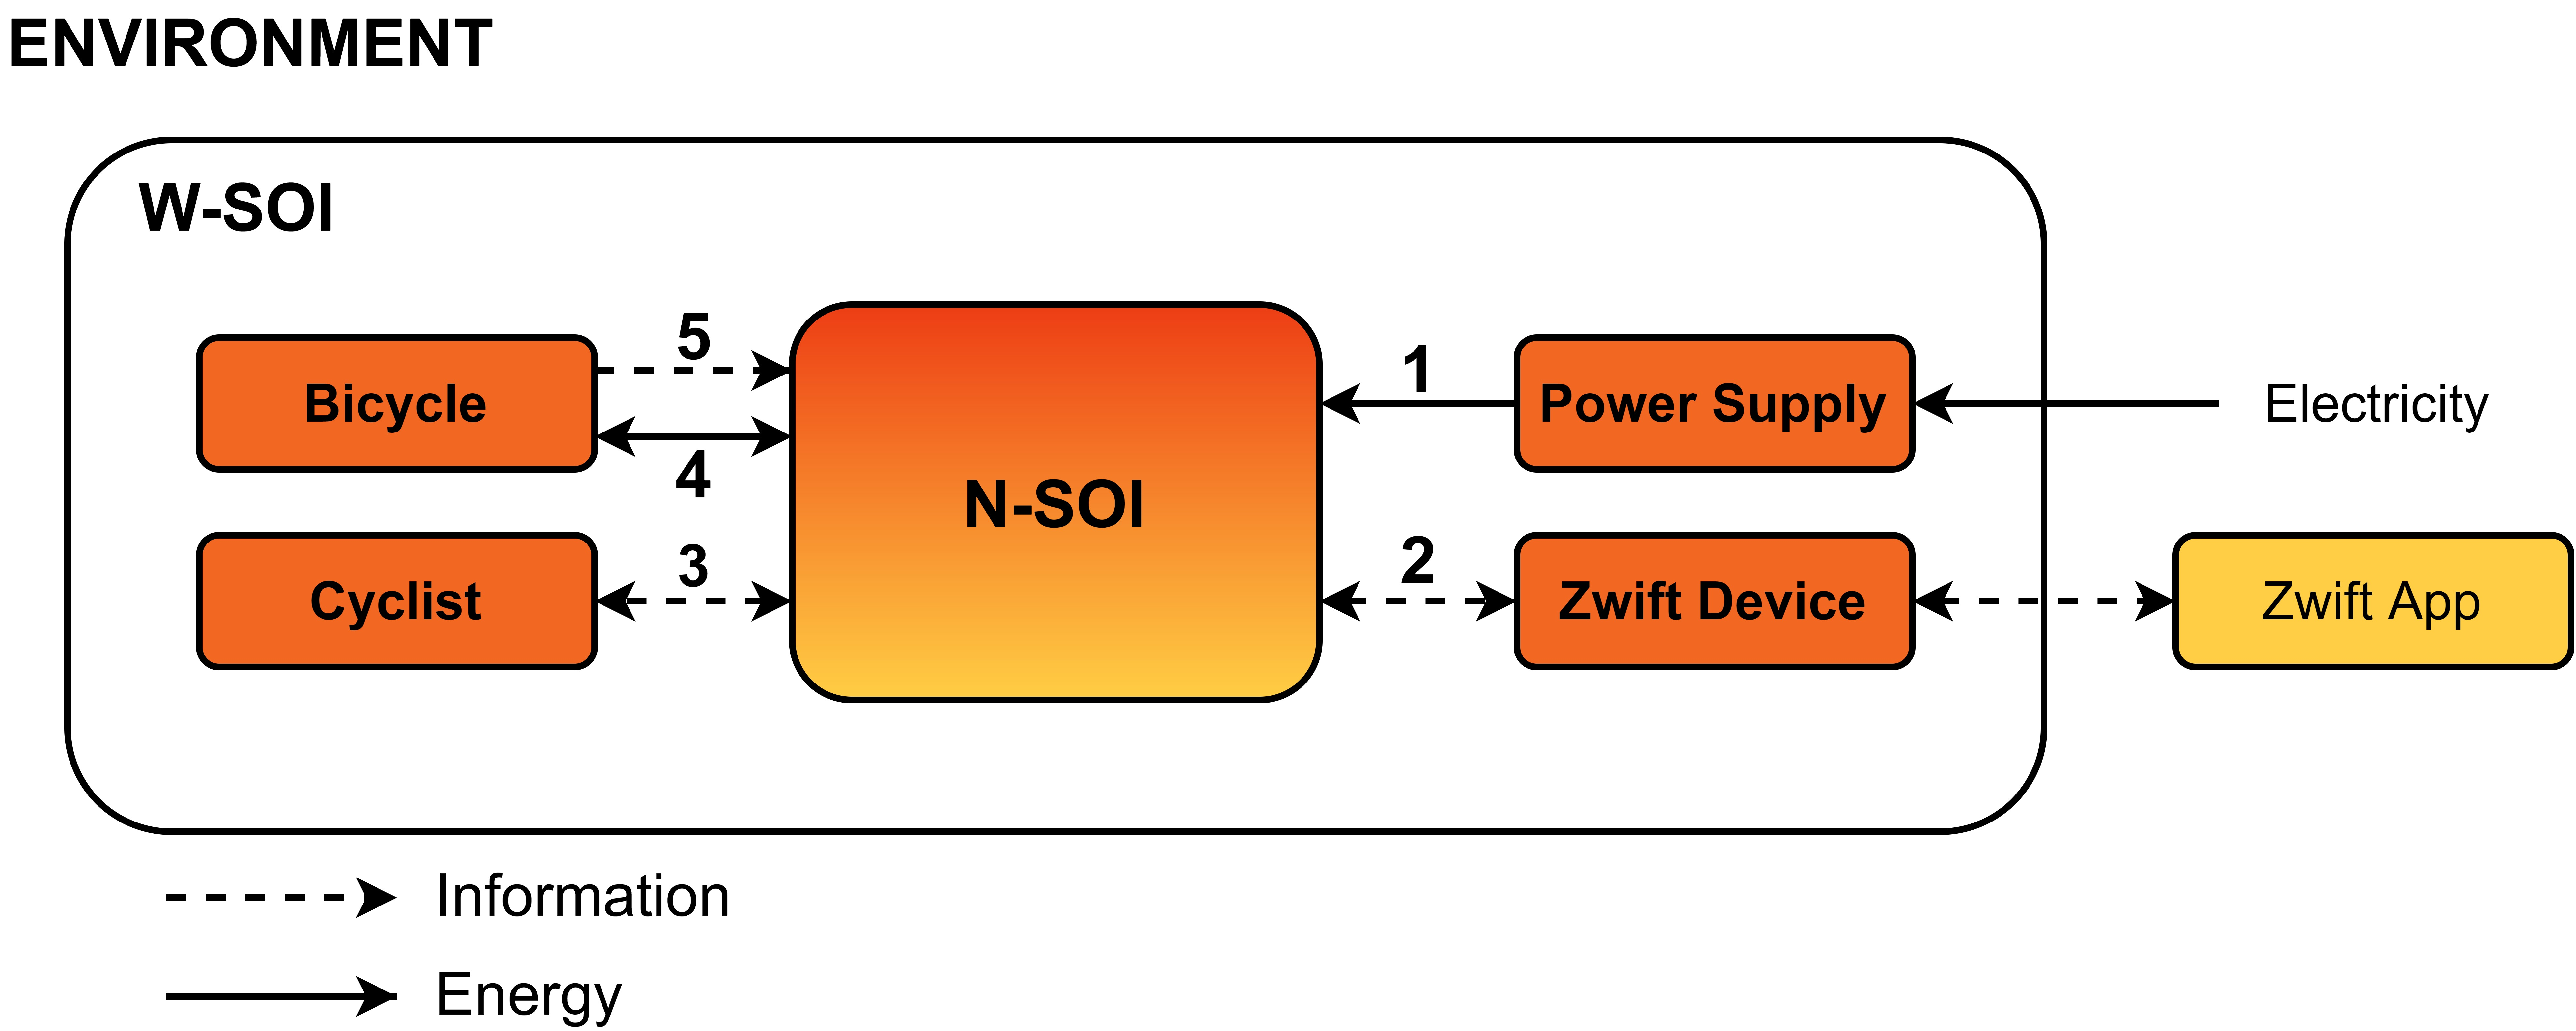
\includegraphics[width=\textwidth]{SOI.jpg}
		\caption{Concept Boundary of Interest}
		\label{fig:soi}
	\end{center}
\end{figure}

The interfaces between elements shown in Figure~\ref{fig:soi} are explained in Table~\ref{tab:links}, and clarified in the following subsections.

\begin{table}[H]
	\renewcommand{\arraystretch}{\tablestretch}
	\centering
	\caption{Concept Boundary Interfaces}
	\begin{tabularx}{\textwidth}{p{1.5cm} X p{4cm}}
		\toprule
		Interface & Description                                           & Type               \\
		\midrule
		1         & \capitalisefmtwords{Power delivery to platform}       & Electrical Energy  \\
		2         & \ac{ble} with \ac{ftms} implementation                & Communication Info \\
		3         & \capitalisefmtwords{User inputs and feedback to user} & User Info          \\
		4         & \capitalisefmtwords{Resistance applied to bicycle}    & Energy Losses      \\
		5         & \capitalisefmtwords{Sensor readings of cycling data}  & Sensor Info        \\
		\bottomrule
	\end{tabularx}
	\label{tab:links}
\end{table}

\subsubsection{2: \ac{ble} with \ac{ftms} implementation}
It was decided to keep the platform completely separate from the device that will be running the Zwift application, as this will allow th platform to easily be used by any other device without requiring any additional modifications.\ac{ble} was chosen as the communication protocol as this is what is available on most consumer electronic devices that Zwift is expected to operate on, and will thus not need an external unit to communicate with the platform.

\subsubsection{\ac{nsoi} Design}

In order to meet the requirements specified above, a \textit{roller trainer} was identified as the platform that would achieve the most desirable outcome. Roller trainers would allow for use with any existing bicycle configuration and a wider range of wheel diameters and wheelbases, without requiring the cyclist to buy or attach any additional components. The solution does however add some complexity to the use of the platform, as it requires additional skill and experience in order to efficiently use roller trainer platforms.

The resistance of the platform will be controlled by an \ac{ecb}, as this would allow for repeatable and frictionless braking torque applied to the rear roller of the trainer. This will accurately simulate outside rolling conditions, as smooth acceleration would be required at high braking torques to avoid the bicycle wheel slipping, similar to what would happen in outside riding conditions.

\section{Concept Evaluation}
\label{sec:eval}

\begin{table}[H]
	\renewcommand{\arraystretch}{\tablestretch}
	\centering
	\caption{Concept Requirement Fulfilment Analysis}
	\begin{tabularx}{\textwidth}{p{1cm} >{\raggedright}X >{\raggedright\arraybackslash}p{1.5cm}}
		\toprule
		Target                 & \multicolumn{1}{c}{Proposed Solution}                                             & Level of Success \\
		\midrule
		FER~\ref{FR:ble}       & \ac{ble} \capitalisefmtwords{communication with device running Zwift application} & Pass             \\
		FER~\ref{FR:wheel}     & \capitalisefmtwords{Roller trainers allow for wider range of wheel diameters}     & Pass             \\
		FER~\ref{FR:speed}     & \capitalisefmtwords{Speed sensors implemented on rollers}                         & Pass             \\
		PER~\ref{PR:wheelbase} & \capitalisefmtwords{Rollers allow for adjustable wheelbase lengths}               & Pass             \\
		PER~\ref{PR:weight}    & \capitalisefmtwords{Rollers do not require heavy bicycle mounting components}     & Pass             \\
		PER~\ref{PR:speed}     & \capitalisefmtwords{Rollers do not limit the operating speed}                     & Pass             \\
		PER~\ref{PR:27speed}   & \capitalisefmtwords{Rollers function independent of bicycle wheel diameter}       & Pass             \\
		PER~\ref{PR:29speed}   & \capitalisefmtwords{Rollers function independent of bicycle wheel diameter}       & Pass             \\
		PER~\ref{PR:torque}    & \capitalisefmtwords{Eddy current brake applied to rear roller}                    & Pass             \\
		\bottomrule
	\end{tabularx}
	\label{tab:eval}
\end{table}

From the evaluation in Table~\ref{tab:eval}, the concept would achieve the functional and performance requirements that were formulated in Section~\ref{sec:req}. The development of the subsequent sections of the concept into a demonstration model is detailed in the sections to follow.